% Options for packages loaded elsewhere
\PassOptionsToPackage{unicode}{hyperref}
\PassOptionsToPackage{hyphens}{url}
%
\documentclass[
]{article}
\usepackage{lmodern}
\usepackage{amssymb,amsmath}
\usepackage{ifxetex,ifluatex}
\ifnum 0\ifxetex 1\fi\ifluatex 1\fi=0 % if pdftex
  \usepackage[T1]{fontenc}
  \usepackage[utf8]{inputenc}
  \usepackage{textcomp} % provide euro and other symbols
\else % if luatex or xetex
  \usepackage{unicode-math}
  \defaultfontfeatures{Scale=MatchLowercase}
  \defaultfontfeatures[\rmfamily]{Ligatures=TeX,Scale=1}
\fi
% Use upquote if available, for straight quotes in verbatim environments
\IfFileExists{upquote.sty}{\usepackage{upquote}}{}
\IfFileExists{microtype.sty}{% use microtype if available
  \usepackage[]{microtype}
  \UseMicrotypeSet[protrusion]{basicmath} % disable protrusion for tt fonts
}{}
\makeatletter
\@ifundefined{KOMAClassName}{% if non-KOMA class
  \IfFileExists{parskip.sty}{%
    \usepackage{parskip}
  }{% else
    \setlength{\parindent}{0pt}
    \setlength{\parskip}{6pt plus 2pt minus 1pt}}
}{% if KOMA class
  \KOMAoptions{parskip=half}}
\makeatother
\usepackage{xcolor}
\IfFileExists{xurl.sty}{\usepackage{xurl}}{} % add URL line breaks if available
\IfFileExists{bookmark.sty}{\usepackage{bookmark}}{\usepackage{hyperref}}
\hypersetup{
  pdftitle={LeastSquares},
  hidelinks,
  pdfcreator={LaTeX via pandoc}}
\urlstyle{same} % disable monospaced font for URLs
\usepackage[margin=1in]{geometry}
\usepackage{longtable,booktabs}
% Correct order of tables after \paragraph or \subparagraph
\usepackage{etoolbox}
\makeatletter
\patchcmd\longtable{\par}{\if@noskipsec\mbox{}\fi\par}{}{}
\makeatother
% Allow footnotes in longtable head/foot
\IfFileExists{footnotehyper.sty}{\usepackage{footnotehyper}}{\usepackage{footnote}}
\makesavenoteenv{longtable}
\usepackage{graphicx,grffile}
\makeatletter
\def\maxwidth{\ifdim\Gin@nat@width>\linewidth\linewidth\else\Gin@nat@width\fi}
\def\maxheight{\ifdim\Gin@nat@height>\textheight\textheight\else\Gin@nat@height\fi}
\makeatother
% Scale images if necessary, so that they will not overflow the page
% margins by default, and it is still possible to overwrite the defaults
% using explicit options in \includegraphics[width, height, ...]{}
\setkeys{Gin}{width=\maxwidth,height=\maxheight,keepaspectratio}
% Set default figure placement to htbp
\makeatletter
\def\fps@figure{htbp}
\makeatother
\setlength{\emergencystretch}{3em} % prevent overfull lines
\providecommand{\tightlist}{%
  \setlength{\itemsep}{0pt}\setlength{\parskip}{0pt}}
\setcounter{secnumdepth}{-\maxdimen} % remove section numbering
\usepackage[width=\textwidth]{caption}

\title{LeastSquares}
\author{}
\date{\vspace{-2.5em}}

\begin{document}
\maketitle

\hypertarget{introduction}{%
\section{1. Introduction}\label{introduction}}

The \color{blue}
\href{https://www.archive.ics.uci.edu/ml/datasets/Bike+Sharing+Dataset}{dataset}
\color{black} for this project is the ``Bike Sharing Dataset Data Set''
found in the UCI Machine Learning Repository. The dataset contains
hourly count of rental bikes for all of 2011 and 2012 (January 1, 2011
to December 31, 2012) in the Capital Bikeshare System of Washington D.C.
area (Washington-Arlington-Alexandria, DC-VA-MD-WV metropolitan area).
The UCI Machine Learning Repository cites Hadi Fanaee-T from the
``Laboratory of Artificial Intelligence and Decision Support (LIAAD),
University of Porto'' for the compilation of the data.

The dataset is outdated since data is actually available up to November
2020 on Capital Bikeshare's website (as of December 18, 2020), but this
limited dataset will still work for the purposes of demonstrating linear
algebra on a real world dataset.

There are two files included in the dataset: a \texttt{hour.csv} and a
\texttt{day.csv}. We will use the \texttt{hour.csv} for the regression,
since the \texttt{day.csv} is simply just a sumamry of the
\texttt{hour.csv} file. We also made a function that easily converts the
\texttt{hour.csv} to the \texttt{day.csv} called
\texttt{convert\_hour\_to\_day()}.

There are 14 different variables that are in this dataset that are
potentially of interest. Two variables are not useful and immediately
thrown out: \texttt{instant} (this is simply the row number of the
dataset) and \texttt{dteday} (date of the year).

Denote \(x_{n}\) as plausible independent variables and denote \(y_{n}\)
as plausible dependent variables.

\(x_{1}\): \texttt{season} (1: spring, 2: summer, 3: fall, 4: winter)

\(x_{2}\): \texttt{yr} (0: 2011, 1: 2012)

\(x_{3}\): \texttt{mnth} (1 to 12)

\(x_{4}\): \texttt{hour} (0 to 23)

\(x_{5}\): \texttt{holiday} (whether a holiday (0 or 1) from
\color{blue}
\href{https://dchrc.dc.gov/page/holiday-schedule}{this list of holidays}
\color{black} )

\(x_{6}\): \texttt{weekday} (0 to 6)

\(x_{7}\): \texttt{workingday} (1 if weekday and not holiday, 0
otherwise)

\(x_{8}\): \texttt{weathersit}: Weather conditions (1: Clear, Few
clouds, Partly cloudy, Partly cloudy, 2: Mist + Cloudy, Mist + Broken
clouds, Mist + Few clouds, Mist, 3: Light Snow, Light Rain +
Thunderstorm + Scattered clouds, Light Rain + Scattered clouds, 4: Heavy
Rain + Ice Pallets + Thunderstorm + Mist, Snow + Fog)

\(x_{9}\): \texttt{temp} (0-1, normalized temperature in Celsius.
Divided by 41)

\(x_{10}\): \texttt{atemp} (0-1, normalized ``feels like'' temperature
in Celsius. Divided by 50)

\(x_{11}\): \texttt{hum} (percent humidity)

\(x_{12}\): \texttt{windspeed} (0-1, Normalized wind speed. Divided by
67)

\(y_{1}\): \texttt{casual} (count of casual users)

\(y_{2}\): \texttt{registered} (count of registered users)

\(y_{3}\): \texttt{cnt} (count of sum of casual and registered users)

The following least squares regression exercise will try to predict the
\texttt{casual}, \texttt{registered}, or \texttt{cnt} as a function of
the independent variables. Also, we will try some principal components
analysis (PCA) and k-nearest neighbors (kNN) with these variables.

\hypertarget{data-analysis}{%
\subsection{Data Analysis}\label{data-analysis}}

Preliminary data analysis shows that the \texttt{hour} is by far the
most important independent variable for explaining the variation in the
dependent variables. Thus, it is important to know how exactly the
\texttt{hour} variable interacts with \texttt{registered},
\texttt{casual}, and \texttt{cnt}.

We also found that it makes sense to treat \texttt{hour} as a
categorical variable (treat \texttt{hour} as 23 independent dummy
variables (0 or 1 for each variable), one for each hour minus the
constant term), but in this case, we will try to fit \texttt{hour} in
terms of a polynomial curve to demonstrate polynomial fitting with
linear algebra.

A plot of \texttt{hour} on the x-axis and \texttt{registered} or
\texttt{casual} on the y-axis would us some insight of what degree
polynomial for \texttt{hour} we should be looking for.

\begin{figure}
\centering
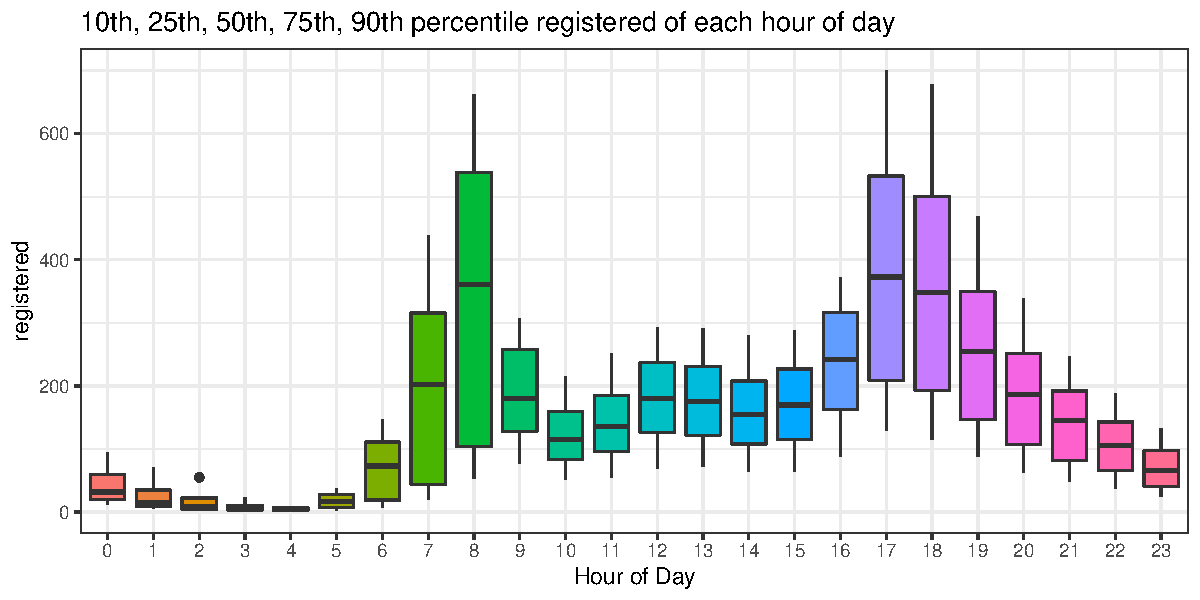
\includegraphics{LeastSquares_files/figure-latex/unnamed-chunk-1-1.pdf}
\caption{Boxplot of registered users for Jan 1, 2011 to December 31,
2011 for each hour of day. The low whisker represents 10th percentile,
the box represents the interquartile range, the top whisker represents
the 90th percentile. For example, with 731 days in the datset, the low
whisker represents the 73rd lowest value.}
\end{figure}

\textbf{Figure 1} for the number of registered users show a trimodal
distribution with three peaks throughout the day. A possible
interpretation of the three peaks is that there is an early peak for the
morning commute, a central peak for lunchtime, and a late peak for the
evening commute. This suggests that we need a high-degree polynomial to
accurately the number of registered users throughout the day. A
six-degree polynomial is the minimum degree that can represent a
trimodal distribution.

\newpage

\begin{figure}
\centering
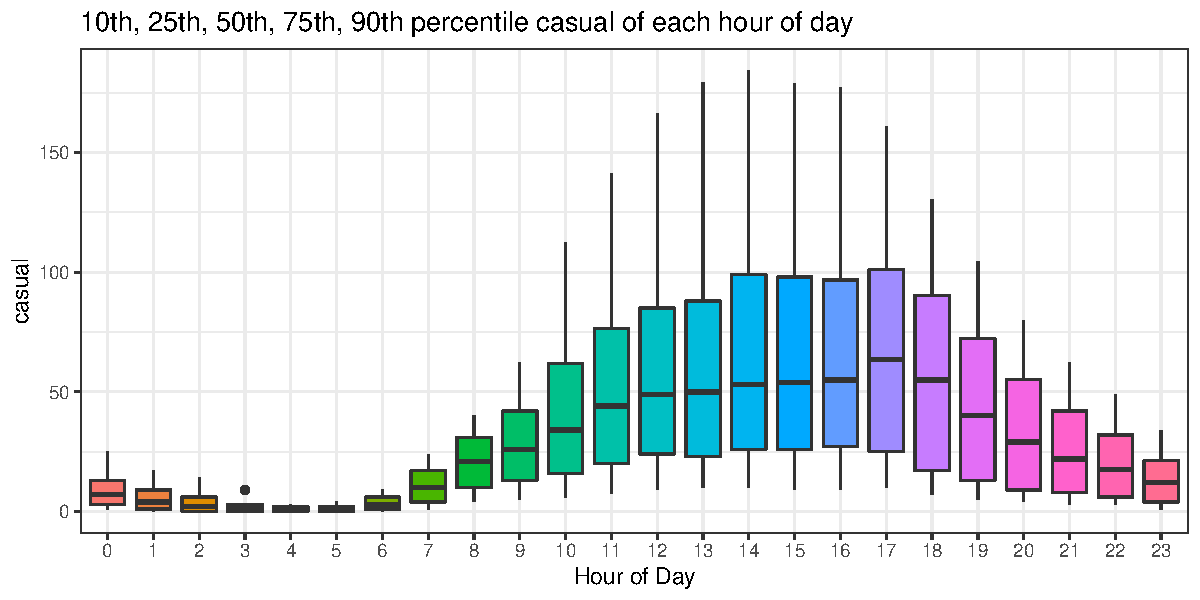
\includegraphics{LeastSquares_files/figure-latex/unnamed-chunk-2-1.pdf}
\caption{Boxplot of casual users for Jan 1, 2011 to December 31, 2011
for each hour of day. The low whisker represents 10th percentile, the
box represents the interquartile range, the top whisker represents the
90th percentile. For example, with 731 days in the datset, the low
whisker represents the 73rd lowest value.}
\end{figure}

\textbf{Figure 2} for the number of casual users show a single peak
distribution. A possible interpretation of this is that casual users are
tourists that don't commute. Tourists are not up early in the morning
and most things to do for tourists occur in the afternoon. Thus, the
peak occurs at around 12 PM-6 PM. A two-degree polynomial is potentially
sufficient to represent the number of casual users throughout the day.

\textbf{Figure 1} and \textbf{Figure 2} show significant variation so
that it is clear that the hour of the day is not the only variable
influencing how many users there are for this bike sharing system. We
can plot at the number of users for each day for further information.

\begin{figure}
\centering
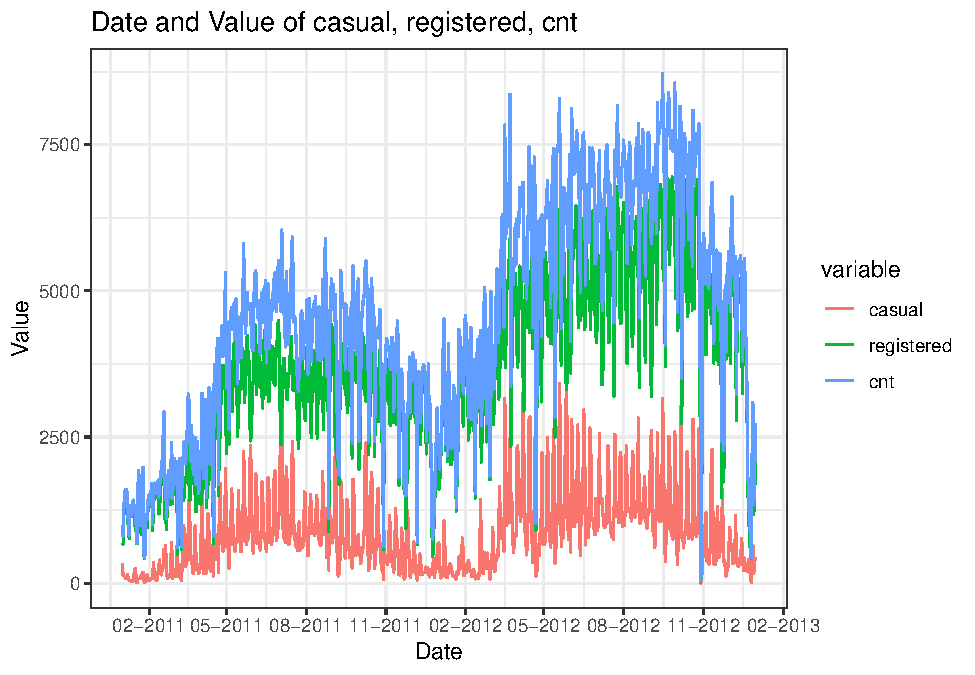
\includegraphics{LeastSquares_files/figure-latex/unnamed-chunk-3-1.pdf}
\caption{Number of casual, registered, and sum of casual and registered
for all 731 days in the dataset}
\end{figure}

\textbf{Figure 3} shows both variation through the year and an increase
in number of users from 2011 to 2012. This makes sense if this Capital
Bike-Sharing was still a developing system in 2011 and not yet a mature
system where the market is already saturated. Thus, we want to include a
variable in our least squares regression model that includes controls
for seasonal variation and the year. This would be \texttt{season} and
\texttt{yr} from the list of \(x_{n}\). It turns out that the
\texttt{weekday} (day of the week) and \texttt{mnth} (month of the year)
do not explain a large additional amount of variation, so they won't be
included in the model.

But \textbf{Figure 3} still shows quite a bit of variation day to day
within each season. There are quite a few weather related variables in
the list of independent variables in the dataset, which would account
for some of the remaining variation.

\begin{figure}
\centering
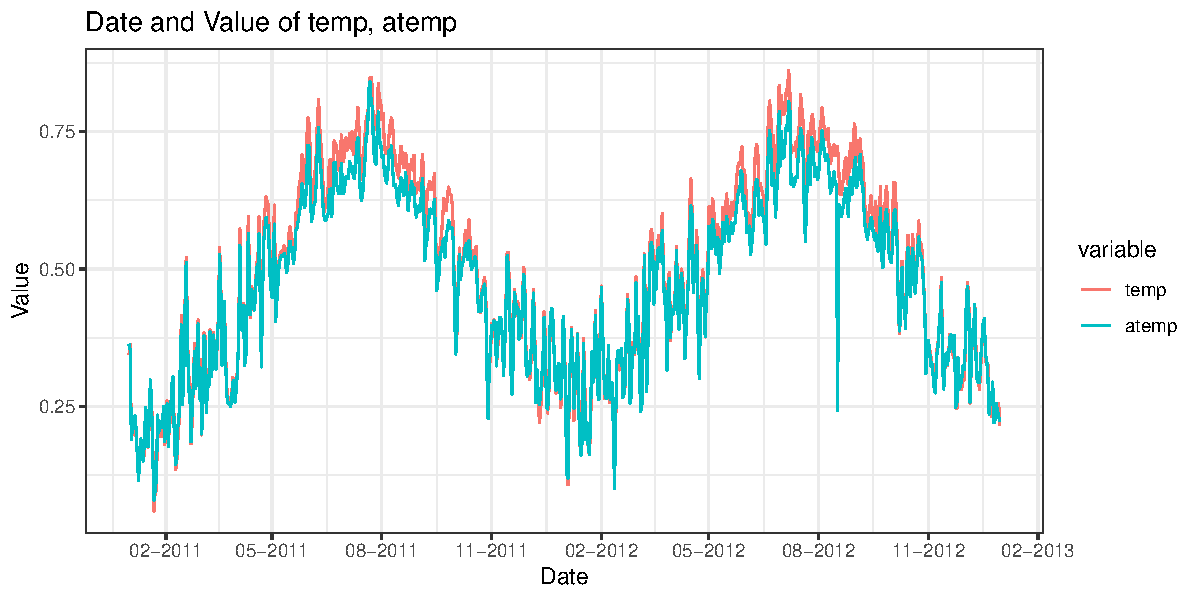
\includegraphics{LeastSquares_files/figure-latex/unnamed-chunk-4-1.pdf}
\caption{Normalized temperature and ``feels like'' temperature for all
731 days in the datset}
\end{figure}

\textbf{Figure 4} shows the average \texttt{temp} (actual temperature)
and \texttt{atemp} (``feels like'' temperature) for each day of the
year. A comparison of \textbf{Figure 3} and \textbf{Figure 4} shows that
temperature shows a strong negative relationship with the number of
bike-sharing users, which makes sense. People do not want to bike when
it is cold outside. These variables have a very high correlation with
each other such that we found it to be sufficient to just add
\texttt{temp}. In fact, \texttt{temp} is good enough to explain most of
the weather-related variation and other variables such as \texttt{wind}
(wind speed) and \texttt{hum} (humidity) are not necessary.

Thus, we choose just \texttt{season}, \texttt{yr}, \texttt{hr}, and
\texttt{temp} as the independent variables and omit the rest of the
variables for the least squares regression model. These are
\(x_{1}, x_{2}, x_{4}\), and \(x_{9}\).

\newpage

\hypertarget{design-matrix}{%
\section{2. Design Matrix}\label{design-matrix}}

The design matrix \(A\) is the matrix that will be used to solve the
equation \(Ax = b\), where \(x\) are the coefficients, often referred to
as the \(\beta\)'s and \(b\) is the dependent variable. It is the matrix
of the explanatory/independent variables.

The design matrix \(A\) will be of \(\mathbb{R}^{17379 \times (n+4)}\),
(where n is the maximum degree of the polynomial for
\(x_{4}\)/\texttt{hour}) since there are 17,379 rows (one for each hour
in the dataset) and there are four variables other than the
\(x_{4}\)/\texttt{hour} variable. The other four variables are the
constant term, \(x_{1}\) (\texttt{season}), \(x_{2}\) (\texttt{yr}), and
\(x_{9}\) (\texttt{temp}).

The following will be the form of our design matrix
\(A \in \mathbb{R}^{17379 \times (n+4)}\) (Note that \(m\) is left the
matrix for simplification, but the of \(m = 17379\)):

\[
A=
  \begin{bmatrix}
    1 & x_{11} & x_{12} & x_{14} & x_{14}^{2} & \dots & x_{14}^{n} & x_{19} \\
    1 & x_{21} & x_{22} & x_{24} & x_{24}^{2} & \dots & x_{24}^{n} & x_{29} \\
    1 & x_{31} & x_{32} & x_{34} & x_{34}^{2} & \dots & x_{34}^{n} & x_{39} \\
    \vdots & \vdots & \vdots & \vdots & \vdots & \ddots & \vdots & \vdots & \\
    1 & x_{m1} & x_{m2} & x_{m4} & x_{m4}^{2} & \dots & x_{m4}^{n} & x_{m9} \\
  \end{bmatrix}
\]

Now the question remaining is the appropriate value of \(n\). We know
that the answer depends on which dependent variable we are using. If
\(b\) is

\begin{longtable}[]{@{}lrrr@{}}
\caption{R-squared values for linear regression of each of value of
\(n\), maximum power of polynomial for \texttt{hour}}\tabularnewline
\toprule
& \(R^{2}_{cnt}\) & \(R^{2}_{casual}\) &
\(R^{2}_{registered}\)\tabularnewline
\midrule
\endfirsthead
\toprule
& \(R^{2}_{cnt}\) & \(R^{2}_{casual}\) &
\(R^{2}_{registered}\)\tabularnewline
\midrule
\endhead
\(x_{4}\) & 0.343 & 0.285 & 0.291\tabularnewline
\(x_{4}+x_{4}^{2}\) & 0.464 & 0.371 & 0.394\tabularnewline
\(x_{4}+x_{4}^{2}+x_{4}^{3}\) & 0.515 & 0.430 & 0.431\tabularnewline
\(x_{4}+x_{4}^{2}+\dots+x_{4}^{4}\) & 0.516 & 0.440 &
0.436\tabularnewline
\(x_{4}+x_{4}^{2}+\dots+x_{4}^{5}\) & 0.530 & 0.446 &
0.464\tabularnewline
\(x_{4}+x_{4}^{2}+\dots+x_{4}^{6}\) & 0.552 & 0.446 &
0.497\tabularnewline
\(x_{4}+x_{4}^{2}+\dots+x_{4}^{7}\) & 0.589 & 0.446 &
0.551\tabularnewline
\(x_{4}+x_{4}^{2}+\dots+x_{4}^{8}\) & 0.599 & 0.446 &
0.565\tabularnewline
\(x_{4}+x_{4}^{2}+\dots+x_{4}^{9}\) & 0.606 & 0.447 &
0.575\tabularnewline
\(x_{4}+x_{4}^{2}+\dots+x_{4}^{10}\) & 0.606 & 0.447 &
0.575\tabularnewline
\(x_{4}+x_{4}^{2}+\dots+x_{4}^{11}\) & 0.613 & 0.447 &
0.585\tabularnewline
\(x_{4}+x_{4}^{2}+\dots+x_{4}^{12}\) & 0.614 & 0.447 &
0.585\tabularnewline
\(x_{4}+x_{4}^{2}+\dots+x_{4}^{13}\) & 0.638 & 0.448 &
0.619\tabularnewline
\(x_{4}+x_{4}^{2}+\dots+x_{4}^{14}\) & 0.638 & 0.448 &
0.619\tabularnewline
\(x_{4}+x_{4}^{2}+\dots+x_{4}^{15}\) & 0.638 & 0.448 &
0.619\tabularnewline
\bottomrule
\end{longtable}

\begin{longtable}[]{@{}lrrrrrrr@{}}
\caption{Comparison of speed (in milliseconds) of custom
design\_matrix() functions with built-in R model.matrix.lm()
function}\tabularnewline
\toprule
expr & min & lq & mean & median & uq & max & neval\tabularnewline
\midrule
\endfirsthead
\toprule
expr & min & lq & mean & median & uq & max & neval\tabularnewline
\midrule
\endhead
design\_matrix() & 19.627 & 20.860 & 29.634 & 22.609 & 30.281 & 172.953
& 100\tabularnewline
design\_matrix\_Cpp() & 7.689 & 8.132 & 10.826 & 8.583 & 10.822 & 30.184
& 100\tabularnewline
model.matrix.lm() & 19.797 & 22.946 & 32.592 & 28.127 & 32.765 & 217.489
& 100\tabularnewline
\bottomrule
\end{longtable}

\hypertarget{normal-equation}{%
\section{3. Normal Equation}\label{normal-equation}}

\begin{longtable}[]{@{}llll@{}}
\caption{Condition number of each value of \(n\) (maximum power of
polynomial for \texttt{hour}) and relative error of normal equations
versus SVD}\tabularnewline
\toprule
\begin{minipage}[b]{0.23\columnwidth}\raggedright
\strut
\end{minipage} & \begin{minipage}[b]{0.15\columnwidth}\raggedright
\(\kappa(A)\)\strut
\end{minipage} & \begin{minipage}[b]{0.15\columnwidth}\raggedright
\(\kappa(A)^{2}\)\strut
\end{minipage} & \begin{minipage}[b]{0.36\columnwidth}\raggedright
Relative error/error message\strut
\end{minipage}\tabularnewline
\midrule
\endfirsthead
\toprule
\begin{minipage}[b]{0.23\columnwidth}\raggedright
\strut
\end{minipage} & \begin{minipage}[b]{0.15\columnwidth}\raggedright
\(\kappa(A)\)\strut
\end{minipage} & \begin{minipage}[b]{0.15\columnwidth}\raggedright
\(\kappa(A)^{2}\)\strut
\end{minipage} & \begin{minipage}[b]{0.36\columnwidth}\raggedright
Relative error/error message\strut
\end{minipage}\tabularnewline
\midrule
\endhead
\begin{minipage}[t]{0.23\columnwidth}\raggedright
\(x_{4}\)\strut
\end{minipage} & \begin{minipage}[t]{0.15\columnwidth}\raggedright
\(8.05 \times 10^{1}\)\strut
\end{minipage} & \begin{minipage}[t]{0.15\columnwidth}\raggedright
\(6.49 \times 10^{3}\)\strut
\end{minipage} & \begin{minipage}[t]{0.36\columnwidth}\raggedright
\(5.87 \times 10^{-12}\)\strut
\end{minipage}\tabularnewline
\begin{minipage}[t]{0.23\columnwidth}\raggedright
\(x_{4}+x_{4}^{2}\)\strut
\end{minipage} & \begin{minipage}[t]{0.15\columnwidth}\raggedright
\(1.45 \times 10^{3}\)\strut
\end{minipage} & \begin{minipage}[t]{0.15\columnwidth}\raggedright
\(2.09 \times 10^{6}\)\strut
\end{minipage} & \begin{minipage}[t]{0.36\columnwidth}\raggedright
\(-1.1 \times 10^{-14}\)\strut
\end{minipage}\tabularnewline
\begin{minipage}[t]{0.23\columnwidth}\raggedright
\(x_{4}+x_{4}^{2}+x_{4}^{3}\)\strut
\end{minipage} & \begin{minipage}[t]{0.15\columnwidth}\raggedright
\(3.01 \times 10^{4}\)\strut
\end{minipage} & \begin{minipage}[t]{0.15\columnwidth}\raggedright
\(9.08 \times 10^{8}\)\strut
\end{minipage} & \begin{minipage}[t]{0.36\columnwidth}\raggedright
\(1.18 \times 10^{-12}\)\strut
\end{minipage}\tabularnewline
\begin{minipage}[t]{0.23\columnwidth}\raggedright
\(x_{4}+x_{4}^{2}+\dots+x_{4}^{4}\)\strut
\end{minipage} & \begin{minipage}[t]{0.15\columnwidth}\raggedright
\(6.46 \times 10^{5}\)\strut
\end{minipage} & \begin{minipage}[t]{0.15\columnwidth}\raggedright
\(4.17 \times 10^{11}\)\strut
\end{minipage} & \begin{minipage}[t]{0.36\columnwidth}\raggedright
\(2.87 \times 10^{-12}\)\strut
\end{minipage}\tabularnewline
\begin{minipage}[t]{0.23\columnwidth}\raggedright
\(x_{4}+x_{4}^{2}+\dots+x_{4}^{5}\)\strut
\end{minipage} & \begin{minipage}[t]{0.15\columnwidth}\raggedright
\(1.42 \times 10^{7}\)\strut
\end{minipage} & \begin{minipage}[t]{0.15\columnwidth}\raggedright
\(2.03 \times 10^{14}\)\strut
\end{minipage} & \begin{minipage}[t]{0.36\columnwidth}\raggedright
\(1.52 \times 10^{-8}\)\strut
\end{minipage}\tabularnewline
\begin{minipage}[t]{0.23\columnwidth}\raggedright
\(x_{4}+x_{4}^{2}+\dots+x_{4}^{6}\)\strut
\end{minipage} & \begin{minipage}[t]{0.15\columnwidth}\raggedright
\(3.59 \times 10^{8}\)\strut
\end{minipage} & \begin{minipage}[t]{0.15\columnwidth}\raggedright
\(1.29 \times 10^{17}\)\strut
\end{minipage} & \begin{minipage}[t]{0.36\columnwidth}\raggedright
Error, Recripocal \(\kappa(A)\): \(5.89 \times 10^{-18}\)\strut
\end{minipage}\tabularnewline
\begin{minipage}[t]{0.23\columnwidth}\raggedright
\(x_{4}+x_{4}^{2}+\dots+x_{4}^{7}\)\strut
\end{minipage} & \begin{minipage}[t]{0.15\columnwidth}\raggedright
\(1.06 \times 10^{10}\)\strut
\end{minipage} & \begin{minipage}[t]{0.15\columnwidth}\raggedright
\(1.12 \times 10^{20}\)\strut
\end{minipage} & \begin{minipage}[t]{0.36\columnwidth}\raggedright
Error, Recripocal \(\kappa(A)\): \(6.14 \times 10^{-21}\)\strut
\end{minipage}\tabularnewline
\begin{minipage}[t]{0.23\columnwidth}\raggedright
\(x_{4}+x_{4}^{2}+\dots+x_{4}^{8}\)\strut
\end{minipage} & \begin{minipage}[t]{0.15\columnwidth}\raggedright
\(3.33 \times 10^{11}\)\strut
\end{minipage} & \begin{minipage}[t]{0.15\columnwidth}\raggedright
\(1.11 \times 10^{23}\)\strut
\end{minipage} & \begin{minipage}[t]{0.36\columnwidth}\raggedright
Error, Recripocal \(\kappa(A)\): \(6.35 \times 10^{-24}\)\strut
\end{minipage}\tabularnewline
\begin{minipage}[t]{0.23\columnwidth}\raggedright
\(x_{4}+x_{4}^{2}+\dots+x_{4}^{9}\)\strut
\end{minipage} & \begin{minipage}[t]{0.15\columnwidth}\raggedright
\(1.10 \times 10^{13}\)\strut
\end{minipage} & \begin{minipage}[t]{0.15\columnwidth}\raggedright
\(1.22 \times 10^{26}\)\strut
\end{minipage} & \begin{minipage}[t]{0.36\columnwidth}\raggedright
Error, Recripocal \(\kappa(A)\): \(6.78 \times 10^{-27}\)\strut
\end{minipage}\tabularnewline
\begin{minipage}[t]{0.23\columnwidth}\raggedright
\(x_{4}+x_{4}^{2}+\dots+x_{4}^{10}\)\strut
\end{minipage} & \begin{minipage}[t]{0.15\columnwidth}\raggedright
\(3.82 \times 10^{14}\)\strut
\end{minipage} & \begin{minipage}[t]{0.15\columnwidth}\raggedright
\(1.46 \times 10^{29}\)\strut
\end{minipage} & \begin{minipage}[t]{0.36\columnwidth}\raggedright
Error, Recripocal \(\kappa(A)\): \(1.29 \times 10^{-29}\)\strut
\end{minipage}\tabularnewline
\begin{minipage}[t]{0.23\columnwidth}\raggedright
\(x_{4}+x_{4}^{2}+\dots+x_{4}^{11}\)\strut
\end{minipage} & \begin{minipage}[t]{0.15\columnwidth}\raggedright
\(1.39 \times 10^{16}\)\strut
\end{minipage} & \begin{minipage}[t]{0.15\columnwidth}\raggedright
\(1.94 \times 10^{32}\)\strut
\end{minipage} & \begin{minipage}[t]{0.36\columnwidth}\raggedright
Error, Recripocal \(\kappa(A)\): \(1.07 \times 10^{-32}\)\strut
\end{minipage}\tabularnewline
\begin{minipage}[t]{0.23\columnwidth}\raggedright
\(x_{4}+x_{4}^{2}+\dots+x_{4}^{12}\)\strut
\end{minipage} & \begin{minipage}[t]{0.15\columnwidth}\raggedright
\(5.38 \times 10^{17}\)\strut
\end{minipage} & \begin{minipage}[t]{0.15\columnwidth}\raggedright
\(2.89 \times 10^{35}\)\strut
\end{minipage} & \begin{minipage}[t]{0.36\columnwidth}\raggedright
Error, Recripocal \(\kappa(A)\): \(7.16 \times 10^{-35}\)\strut
\end{minipage}\tabularnewline
\begin{minipage}[t]{0.23\columnwidth}\raggedright
\(x_{4}+x_{4}^{2}+\dots+x_{4}^{13}\)\strut
\end{minipage} & \begin{minipage}[t]{0.15\columnwidth}\raggedright
\(2.21 \times 10^{19}\)\strut
\end{minipage} & \begin{minipage}[t]{0.15\columnwidth}\raggedright
\(4.86 \times 10^{38}\)\strut
\end{minipage} & \begin{minipage}[t]{0.36\columnwidth}\raggedright
Error, Recripocal \(\kappa(A)\): \(1.13 \times 10^{-37}\)\strut
\end{minipage}\tabularnewline
\begin{minipage}[t]{0.23\columnwidth}\raggedright
\(x_{4}+x_{4}^{2}+\dots+x_{4}^{14}\)\strut
\end{minipage} & \begin{minipage}[t]{0.15\columnwidth}\raggedright
\(5.86 \times 10^{22}\)\strut
\end{minipage} & \begin{minipage}[t]{0.15\columnwidth}\raggedright
\(3.43 \times 10^{45}\)\strut
\end{minipage} & \begin{minipage}[t]{0.36\columnwidth}\raggedright
Error, Recripocal \(\kappa(A)\): \(2.67 \times 10^{-40}\)\strut
\end{minipage}\tabularnewline
\begin{minipage}[t]{0.23\columnwidth}\raggedright
\(x_{4}+x_{4}^{2}+\dots+x_{4}^{15}\)\strut
\end{minipage} & \begin{minipage}[t]{0.15\columnwidth}\raggedright
\(4.51 \times 10^{22}\)\strut
\end{minipage} & \begin{minipage}[t]{0.15\columnwidth}\raggedright
\(2.04 \times 10^{45}\)\strut
\end{minipage} & \begin{minipage}[t]{0.36\columnwidth}\raggedright
Error, Recripocal \(\kappa(A)\): \(2.51 \times 10^{-43}\)\strut
\end{minipage}\tabularnewline
\bottomrule
\end{longtable}

\begin{longtable}[]{@{}lrrrrrrr@{}}
\caption{Comparison of speed (in milliseconds) of solving \(Ax = b\)
where \(A \in \mathbb{R}^{17379 \times 7}\) using normal equations
implemented in R vs Rcpp (C++)}\tabularnewline
\toprule
expr & min & lq & mean & median & uq & max & neval\tabularnewline
\midrule
\endfirsthead
\toprule
expr & min & lq & mean & median & uq & max & neval\tabularnewline
\midrule
\endhead
normal\_equations(A, b) & 5.976 & 6.734 & 8.806 & 7.379 & 9.161 & 31.031
& 100\tabularnewline
normal\_equations\_Cpp(A, b) & 4.931 & 5.243 & 6.160 & 5.742 & 6.741 &
11.054 & 100\tabularnewline
\bottomrule
\end{longtable}

\hypertarget{qr-decomposition}{%
\section{4. QR Decomposition}\label{qr-decomposition}}

\begin{longtable}[]{@{}lrrrrrrr@{}}
\caption{Comparison of speed (in milliseconds) of solving \(Ax = b\)
where \(A \in \mathbb{R}^{17379 \times 7}\) using QR decomposition
implemented in R vs Rcpp (C++)}\tabularnewline
\toprule
expr & min & lq & mean & median & uq & max & neval\tabularnewline
\midrule
\endfirsthead
\toprule
expr & min & lq & mean & median & uq & max & neval\tabularnewline
\midrule
\endhead
qr.solve(A, b) & 5.391 & 6.532 & 9.216 & 7.226 & 9.042 & 29.765 &
100\tabularnewline
qr\_solve\_Cpp(A, b) & 5.396 & 5.677 & 6.915 & 6.271 & 7.499 & 14.989 &
100\tabularnewline
\bottomrule
\end{longtable}

\hypertarget{singular-value-decomposition}{%
\section{5. Singular Value
Decomposition}\label{singular-value-decomposition}}

\begin{longtable}[]{@{}lrrrrrrr@{}}
\caption{Comparison of speed (in milliseconds) of solving \(Ax = b\)
where \(A \in \mathbb{R}^{17379 \times 7}\) using SVD implemented in R
vs Rcpp (C++)}\tabularnewline
\toprule
expr & min & lq & mean & median & uq & max & neval\tabularnewline
\midrule
\endfirsthead
\toprule
expr & min & lq & mean & median & uq & max & neval\tabularnewline
\midrule
\endhead
svd\_solve(A, b) & 9.523 & 11.059 & 13.821 & 12.049 & 14.157 & 38.720 &
100\tabularnewline
svd\_solve\_Cpp(A, b) & 8.190 & 8.734 & 10.369 & 9.620 & 11.021 & 35.461
& 100\tabularnewline
\bottomrule
\end{longtable}

\begin{longtable}[]{@{}lrrrrrrr@{}}
\caption{Comparison of speed (in milliseconds) of solving \(Ax = b\)
where \(A \in \mathbb{R}^{17379 \times 7}\) using normal equations, QR
decomposition, and SVD implemented in R vs Rcpp (C++)}\tabularnewline
\toprule
expr & min & lq & mean & median & uq & max & neval\tabularnewline
\midrule
\endfirsthead
\toprule
expr & min & lq & mean & median & uq & max & neval\tabularnewline
\midrule
\endhead
normal\_equations(A, b) & 6.058 & 7.092 & 9.496 & 7.808 & 9.591 & 31.948
& 100\tabularnewline
normal\_equations\_Cpp(A, b) & 4.906 & 5.231 & 6.371 & 5.875 & 6.940 &
13.142 & 100\tabularnewline
qr.solve(A, b) & 5.518 & 6.950 & 12.626 & 8.000 & 10.654 & 235.429 &
100\tabularnewline
qr\_solve\_Cpp(A, b) & 5.440 & 5.849 & 7.795 & 6.411 & 7.675 & 73.373 &
100\tabularnewline
svd\_solve(A, b) & 9.636 & 12.183 & 16.248 & 14.263 & 18.056 & 66.454 &
100\tabularnewline
svd\_solve\_Cpp(A,b) & 8.298 & 9.201 & 11.884 & 10.529 & 12.813 & 57.141
& 100\tabularnewline
\bottomrule
\end{longtable}

\begin{longtable}[]{@{}lrrrrrrr@{}}
\caption{Comparison of speed (in milliseconds) of solving \(Ax = b\)
where \(A \in \mathbb{R}^{17379 \times 11}\) using QR decomposition or
SVD implemented in R vs Rcpp (C++)}\tabularnewline
\toprule
expr & min & lq & mean & median & uq & max & neval\tabularnewline
\midrule
\endfirsthead
\toprule
expr & min & lq & mean & median & uq & max & neval\tabularnewline
\midrule
\endhead
qr.solve(A, b) & 10.327 & 12.829 & 18.078 & 15.083 & 20.989 & 55.218 &
100\tabularnewline
qr\_solve\_Cpp(A, b) & 11.714 & 12.863 & 16.213 & 14.736 & 17.559 &
41.542 & 100\tabularnewline
svd\_solve(A, b) & 20.475 & 25.185 & 33.355 & 30.504 & 37.977 & 78.544 &
100\tabularnewline
svd\_solve\_Cpp(A,b) & 17.806 & 19.218 & 24.953 & 20.885 & 23.506 &
140.779 & 100\tabularnewline
\bottomrule
\end{longtable}

\hypertarget{final-regression-model}{%
\section{6. Final Regression Model}\label{final-regression-model}}

\(y_{1} = \beta_{0} + \beta_{1}x_{1} + \beta_{2}x_{2} + \beta_{3}x_{4} + \beta_{4}x_{4}^{2} + \beta_{5}x_{4}^{3} + \beta_{6}x_{9}\)

\(y_{3} = \beta_{0} + \beta_{1}x_{1} + \beta_{2}x_{2} + \beta_{3}x_{4} + \beta_{4}x_{4}^{2} + \beta_{5}x_{4}^{3} + \beta_{6}x_{4}^{4} + \beta_{7}x_{4}^{5} + \beta_{8}x_{4}^{6} + \beta_{9}x_{4}^{7} + \beta_{10}x_{9}\)

With the data inputed, we have

\(y_{1} = -42.145 + 0.6875x_{1} + 12.887x_{2} - 4.859x_{4} + 1.275x_{4}^{2} - 0.047x_{4}^{3} + 89.528x_{9}\)

\(y_{3} = -145.05 + 17.18x_{1} + 88.57x_{2} + 29.45x_{4} - 63.199x_{4}^{2} + 24.27x_{4}^{3} - 3.62x_{4}^{4} + 0.258x_{4}^{5} - 0.0088x_{4}^{6} + 0.000116x_{4}^{7} + 243.131x_{9}\)

Note that
\(\frac{1}{n}\sum_{i=1}^{n} x_{1} = \bar{x_{1}} = 2.50164, \frac{1}{n}\sum_{i=1}^{n} x_{2} = \bar{x_{2}} = 0.5025606, \frac{1}{n}\sum_{i=1}^{n} x_{8} = \bar{x_{8}} = 0.4970\).

\begin{figure}
\centering
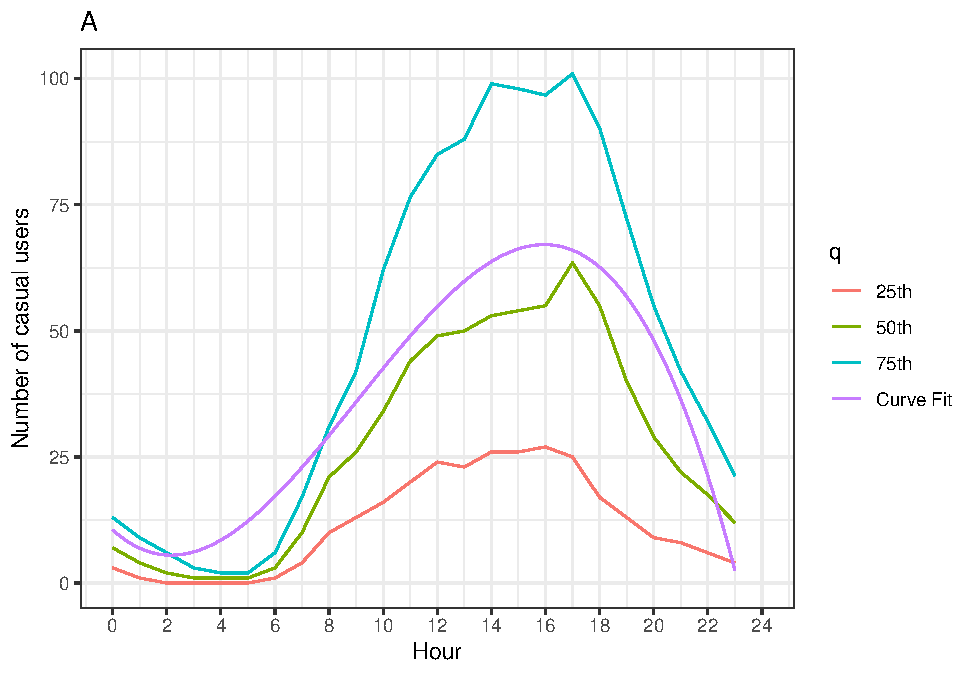
\includegraphics{LeastSquares_files/figure-latex/unnamed-chunk-14-1.pdf}
\caption{A}
\end{figure}

\begin{figure}
\centering
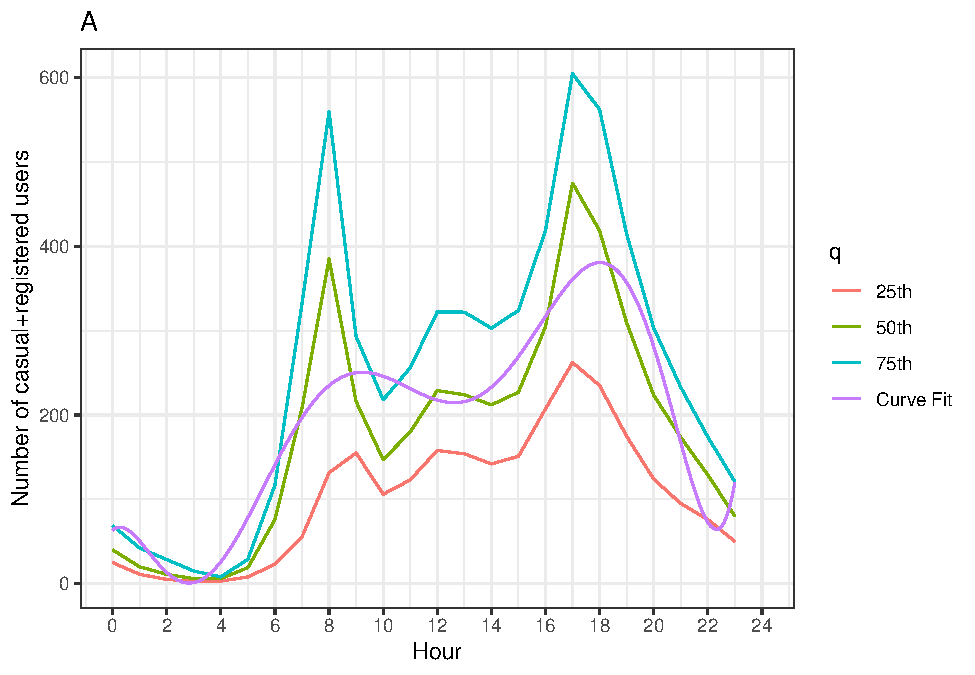
\includegraphics{LeastSquares_files/figure-latex/unnamed-chunk-15-1.pdf}
\caption{A}
\end{figure}

\end{document}
